\documentclass[12pt]{article}

\usepackage[utf8]{inputenc} 
\usepackage[T1]{fontenc} 
\usepackage{graphicx}
\usepackage{geometry}

\geometry{top=2.5cm, bottom=2.5cm, left=2.5cm, right=2.5cm} % Setze Seitenränder
\setlength{\parindent}{0pt}   % Deaktiviert Einrücken
\setlength{\parskip}{1em}     % Abstand zwischen Absätzen

\begin{document}

\title{\textbf{Werkzeuge für das wissenschaftliche Arbeiten}\\\large Python for Machine Learning and Data Science}

\date{\vspace{-1cm}\hfill Abgabe: 15.12.2023}
\maketitle

\vspace{-1cm}
\hrule

\tableofcontents


\section{Projektaufgabe}
In dieser Aufgabe beschäftigen wir uns mit Objektorientierung in Python. Der Fokus liegt auf der Implementierung einer Klasse, dabei nutzen wir insbesondere auch Magic Methods.

\renewcommand{\figurename}{Abbildung}
\begin{figure}[h!]
    \centering
    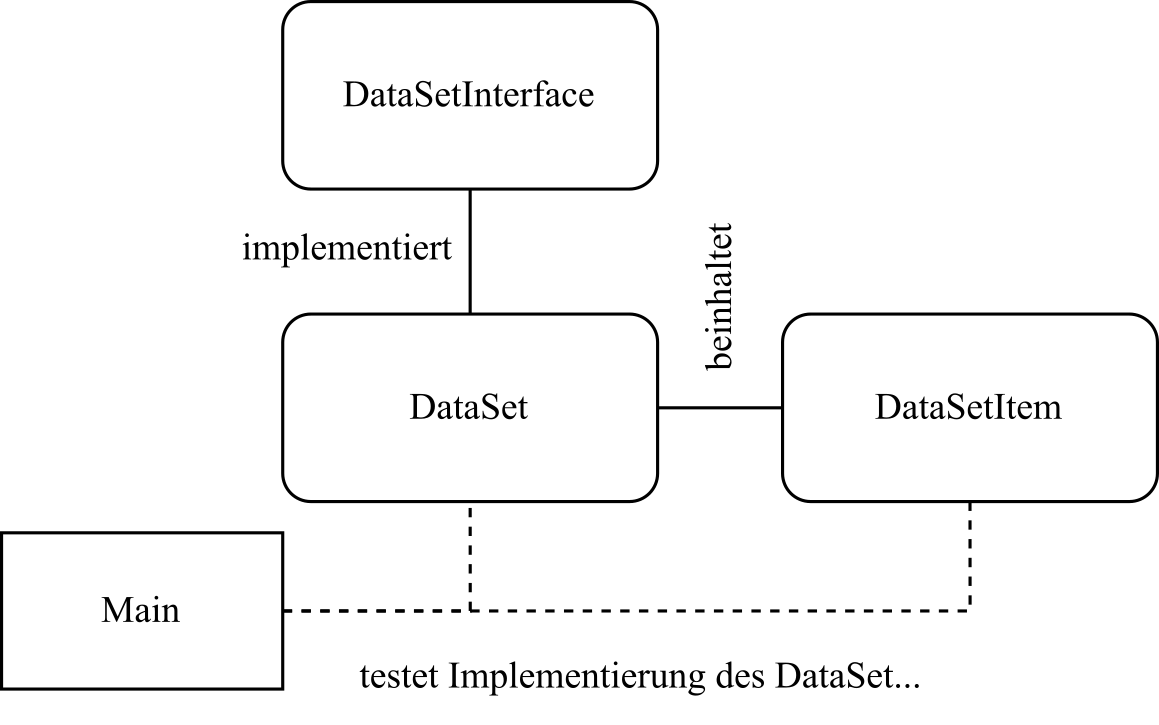
\includegraphics[scale=0.9]{./../diagram/new_diagram.png}
    \caption{Darstellung der Klassenbeziehungen}
\end{figure}

\subsection{Einleitung}
Ein Datensatz besteht aus mehreren Daten, ein einzelnes Datum wird durch ein Objekt der Klasse \texttt{DataSetItem} repräsentiert. Jedes Datum hat einen Namen (Zeichenkette), eine ID (Zahl) und beliebigen Inhalt.

Nun sollen mehrere Daten, Objekte vom Typ \texttt{DataSetItem}, in einem Datensatz zusammengefasst werden. Es gibt eine Klasse \texttt{DataSetInterface}, die die Schnittstelle definiert und die Operationen eines Datensatzes angibt. Bisher fehlt jedoch noch die Implementierung eines Datensatzes mit allen Operationen.

Implementieren Sie eine Klasse \texttt{DataSet} als eine Unterklasse von \texttt{DataSetInterface}.

\subsection{Aufbau}
Es gibt drei Dateien, \texttt{dataset.py}, \texttt{main.py} und \texttt{implementation.py}. In der \texttt{dataset.py} befinden sich die Klassen \texttt{DataSetInterface} und \texttt{DataSetItem}, in der Datei \texttt{implementation.py} muss die Klasse \texttt{DataSet} implementiert werden. Die Datei \texttt{main.py} nutzt die Klassen \texttt{DataSet} und \texttt{DataSetItem} aus den jeweiligen Dateien und testet die Schnittstelle und Operationen von
\texttt{DataSetInterface}.

\subsection{Methoden}
Bei der Klasse \texttt{DataSet} sind insbesondere folgende Methoden zu implementieren, die genaue Spezifikation finden Sie in der \texttt{dataset.py}:

\begin{enumerate}
    \item \texttt{\_\_setitem\_\_}(self, name, id\_content) - Hinzufügen eines Datums, mit Name, ID und Inhalt.
    \item \texttt{\_\_iadd\_\_}(self, item) - Hinzufügen eines \texttt{DataSetItem}.
    \item \texttt{\_\_delitem\_\_}(self, name) - Löschen eines Datums basierend auf dem Namen.
    \item \texttt{\_\_contains\_\_}(self, name) - Prüfung, ob ein Datum mit diesem Namen im Datensatz vorhanden ist.
    \item \texttt{\_\_getitem\_\_}(self, name) - Abrufen eines Datums über seinen Namen.
    \item \texttt{\_\_and\_\_}(self, dataset) - Schnittmenge zweier Datensätze bestimmen und als neuen Datensatz zurückgeben.
    \item \texttt{\_\_or\_\_}(self, dataset) - Vereinigungen zweier Datensätze bestimmen und als neuen Datensatz zurückgeben.
    \item \texttt{\_\_iter\_\_}(self) - Iteration über alle Daten des Datensatzes.
    \item \texttt{filtered\_iterate}(self, filter) - Gefilterte Iteration über den Datensatz, wobei eine Lambda-Funktion als Filter dient.
    \item \texttt{\_\_len\_\_}(self) - Anzahl der Daten im Datensatz abrufen.
\end{enumerate}

\section{Abgabe}
Programmieren Sie die Klasse \texttt{DataSet} in der Datei \texttt{implementation.py} zur Lösung der oben beschriebenen Aufgabe im VPL. Sie können auch direkt auf Ihrem Computer programmieren, dazu finden Sie alle drei benötigten Dateien zum Download im Moodle.

Das VPL nutzt den gleichen Code, wobei \texttt{main.py} um weitere Testfälle und Überprüfungen erweitert wurde. Die Überprüfungen dienen dazu, sicherzustellen, dass Sie die richtigen Klassen nutzen.

\vspace{1cm}
\hrule
\vspace{0.2cm}

\textit{* Dateien befinden sich im Ordner "/code/" dieses Git-Repositories.}

\end{document}